\chapter{Drawing on Images}
\label{chapter:drawingOnImages}

\newcounter{drawingOnImages}
\setcounter{drawingOnImages}{0}
\stepcounter{drawingOnImages}

\section{Example \thedrawingOnImages}
\stepcounter{drawingOnImages}

\begin{figure}[H]
	\begin{center}
		\scalebox{1}{
			\begin{tikzpicture}
			
			%Inserisco i nodi che poi conterrano l'immagine
			\node (auto) at (-6,0) [rectangle, minimum width=1cm, minimum height=1cm, label=\textbf{Haar cascade}] {\includegraphics[scale=0.25]{figure/Haar_rilevazione.png}};
			
			\node (auto) at (0,0) [rectangle, minimum width=1cm, minimum height=1cm, label=\textbf{HOG}] {\includegraphics[scale=0.25]{figure/HOG_rilevazione.png}};
			
			\end{tikzpicture}
		}
	\end{center}

\end{figure}

\section{Example \thedrawingOnImages}
\stepcounter{drawingOnImages}

\begin{figure}[H]
	\begin{center}
		\begin{tikzpicture}
		
		%Disegno il sistema di riferimento
		\draw[dashed] (0,0) coordinate -- (0,1.3) coordinate;
		\draw[->] (0,1.3) coordinate -- (0,5) coordinate node[above left]{$Y$};
		\draw[dashed] (0,0) coordinate -- (1.6,0) coordinate;
		\draw[->] (1.6,0) coordinate -- (3,0) coordinate node[above right]{$X$};
		\draw[dashed] (0,0) coordinate -- (-0.5,-0.5) coordinate;
		\draw[->] (-0.5,-0.5) coordinate -- (-2,-2) coordinate node[above left]{$Z$};
		\draw[dashed] (0,0) coordinate -- (1,1) coordinate;
		\draw[-] (1,1) coordinate -- (3,3) coordinate node[below right]{$-Z$};
		\draw[-] (-1.6,0) coordinate -- (-6,0) coordinate;
		
		%Disegno pre proiezioni della camera
		\draw[dashed] (-5,-1) coordinate -- (-5,4) coordinate;
		\draw[dashed] (-4,0) coordinate -- (-5,-1) coordinate;
		\draw[dashed] (-5,-1) coordinate -- (-1,-1) coordinate;
		
		%Disegno l'angolo
		\draw[dashed] (-5,-1) coordinate (a) -- (0,0) coordinate (b) -- (-5,4) coordinate (c)
		pic["$\mathbf{\beta}$", draw, <-, angle eccentricity=1.2, angle radius=2.5cm, line width=1.25pt]{angle=c--b--a};
		
		\draw[dashed] (-4,0) coordinate (d) -- (0,0) coordinate (e);
		
		\draw[dashed] pic["$\mathbf{\alpha}$", draw, ->, angle eccentricity=1.2, angle radius=3.25cm, line width=1.25pt]{angle=d--e--a};
		
		\draw (-3,2.7) coordinate node[above]{$r$};
		
		%Inserisco i nomi
		\draw (-6,5) coordinate node[above]{$\mathbf{Camera}$};
		\draw (2,-1) coordinate node[above left]{$\mathbf{Car}$};
		
		%Inserisco fotocamera ed auto
		%TRIM = sinistra sotto destra sopra
		\node at (-5,5) []{\includegraphics[scale=0.15, trim=17cm 18cm 15cm 45cm]{pdf/Fotocamera.pdf}};
		\node at (2,-1) []{\includegraphics[scale=0.15, trim=17cm 3cm -12cm 45cm]{pdf/Auto.pdf}};
		
		
		\end{tikzpicture}
	\end{center}
	
\end{figure}


\section{Example \thedrawingOnImages}
\stepcounter{drawingOnImages}

\begin{figure}[H]
	\begin{center}
		\scalebox{1}{
			\begin{tikzpicture}
			
			%Rappresento gli angoli sul sistema di riferimento inerziale
			\draw[<-] (0.15,2.3) arc (-25:-110:0.30cm) node[above left]{$\psi$};
			\draw[<-] (-1.9,-1.085) arc (35:-150:0.30cm);
			\draw (-1.7,-1.3) node[below]{$\phi$};
			\draw[<-] (1.8,-1.125) arc (115:-100:0.30cm) node[below right]{$\theta$};
			
			%Inserisco il sistema di riferimento assi-corpo
			\draw[->] (0,0) coordinate -- (0,3) coordinate node[anchor=west]{$u_{z}$};
			\draw[->] (0,0) coordinate -- (-2.5,-1.625) coordinate node[below left]{$u_{x}$};
			\draw[->] (0,0) coordinate -- (2.5,-1.625) coordinate node[below right]{$u_{y}$};
			\draw (-0.05,0.9) node[below right]{$O_{ABC}$};
			
			%Inserisco l'esacottero
			\node (esacottero) at (0,-0.25) [text centered]{\includegraphics[scale=0.15]{figure/esacottero_CAD_trasparente.png}};
			
			%Inserisco gli archi per le Omega
			\draw[<-] (-1.475,-0.385) arc (-25:-100:0.30cm);
			\draw[->] (-1.78,0.7) arc (-35:-110:0.30cm);
			\draw[<-] (-0.365,1.275) arc (-25:-100:0.30cm);
			\draw[->] (1.325,1.175) arc (-45:-110:0.30cm);
			\draw[<-] (2.395,0.3725) arc (-25:-100:0.30cm);
			\draw[->] (1.1625,-0.5725) arc (-25:-100:0.30cm);
			
			%Disegno i vettori delle forze
			\draw[->] (-1.675,-0.685) coordinate -- (-1.675,-0.185) node[left]{$\Omega_1$};
			\draw[->] (-1.98,0.4) coordinate -- (-1.98,0.9) node[left]{$\Omega_6$};
			\draw[->] (-0.565,0.975) coordinate -- (-0.565,1.475) node[left]{$\Omega_5$};
			\draw[->] (1.165,0.875) coordinate -- (1.165,1.375) node[left]{$\Omega_4$};
			\draw[->] (2.195,0.0725) coordinate -- (2.195,0.5725) node[right]{$\Omega_3$};
			\draw[->] (0.9625,-0.9725) coordinate -- (0.9625,-0.4725) coordinate;
			\draw (1.4625,-0.7725) node[above]{$\Omega_2$};
			
			%Rappresento gli angoli sul sistema di riferimento inerziale
			\draw[<-] (-4.3,-1.5) arc (-25:-110:0.30cm) node[left]{$\psi$};
			\draw[<-] (-3.15,-4) arc (55:-110:0.30cm) node[below right]{$\theta$};
			\draw[<-] (-6.1,-3.8) arc (115:-100:0.30cm) node[below right]{$\phi$};
			
			%Inserisco il sistema di riferimento inerziale
			\draw[->] (-4.5,-3) coordinate -- (-4.5,0) coordinate node[anchor=east]{$u_{z}$};
			\draw[->] (-4.5,-3) coordinate -- (-7,-5) coordinate node[below right]{$u_{x}$};
			\draw[->] (-4.5,-3) coordinate -- (-2.5,-5) coordinate node[below left]{$u_{y}$};
			\draw (-4.5,-3) node[right]{$O_{FI}$};
			
			\end{tikzpicture}
		}
	\end{center}
	
\end{figure}

\section{Example \thedrawingOnImages}
\stepcounter{drawingOnImages}

\begin{figure}[H]
	\begin{center}
		\scalebox{1}{
			\begin{tikzpicture}[node distance=2cm]
			
			%Creo i nodi del diagramma di flusso		
			\node (classificatore) at (0,0) [rectangle, draw, text centered, minimum width=2.5cm, minimum height=1cm] {Classifier};
			
			\node (sistemaRiconoscimentoVisi) at (0,-4) [rectangle, draw, text centered, minimum width=2.5cm, minimum height=1cm] {Faces recognition};
			
			\node (endrix) at (-5,-4) [rectangle, minimum width=1cm, minimum height=1cm] {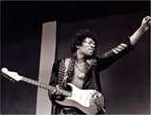
\includegraphics[scale=0.8]{figure/endrix.png}};
			
			\node (endrixRiconosciuto) at (5,-4) [rectangle, minimum width=2cm, minimum height=1cm] {\includegraphics[scale=0.8]{figure/endrixNoto.png}};
			
			\node (falsiPositivi) at (5,1) [rectangle, minimum width=2cm, minimum height=1cm, label=Falsi Positivi] {\includegraphics[scale=1]{figure/falsiPositiviPhoto.png}};
			
			\node (dataSet) at (-5,1) [rectangle, minimum width=2cm, minimum height=1cm, label=Dataset Iniziale] {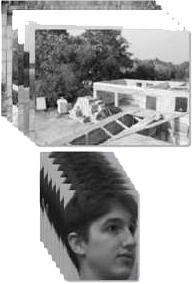
\includegraphics[scale=0.6]{figure/dataSet.png}};
			
			%Collego i nodi
			\draw [->] (classificatore.south) -- (sistemaRiconoscimentoVisi.north);
			
			\draw [->] (endrix.east) -- (sistemaRiconoscimentoVisi.west);
			
			\draw [->] (endrixRiconosciuto.north) -- (falsiPositivi.south);
			
			\draw [->] (sistemaRiconoscimentoVisi.east) -- (endrixRiconosciuto.west);
			
			\draw [->] (dataSet) to [out=0,in=90] (classificatore);
			\draw [->] (falsiPositivi) to [out=180,in=90] (classificatore);
			
			\end{tikzpicture}
		}
	\end{center}
\end{figure}

\section{Example \thedrawingOnImages}
\stepcounter{drawingOnImages}

\begin{figure}[H]
	\begin{center}
		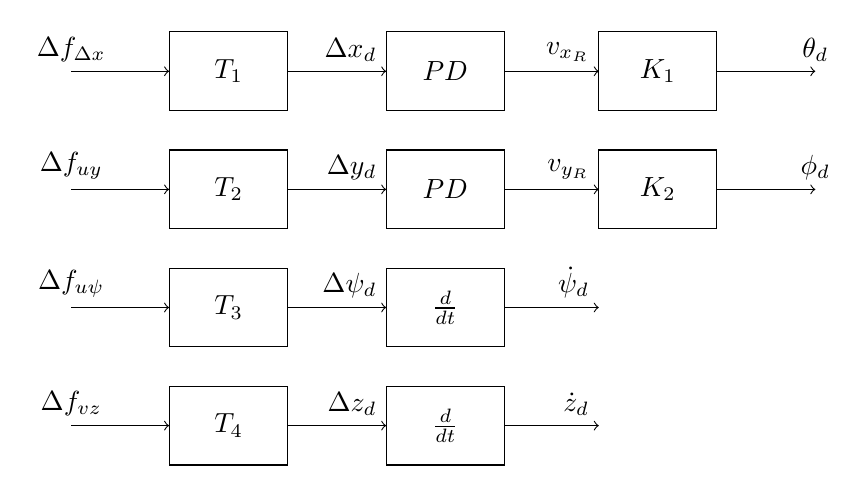
\begin{tikzpicture}
		
		%Disegno i nodi del primo schema
		\node (primaTrasformazione) at (-2,0) [draw, rectangle, minimum width=1.5cm, minimum height=1cm, text centered]{$T_1$};
		
		\node (primoPD) at (0.75,0) [draw, text centered, minimum width=1.5cm, minimum height=1cm]{$PD$};
		
		\node (primoK) at (3.45,0) [draw, text centered, minimum width=1.5cm, minimum height=1cm]{$K_1$};
		
		%Disegno i collegamenti
		\draw[->] (-4,0) coordinate node[above]{$\Delta f_{\Delta x}$} -- (primaTrasformazione.west);
		
		\draw[->] (primaTrasformazione.east) -- (0,0) coordinate node[above left]{$\Delta x_d$};
		
		\draw[->] (primoPD.east) -- (2.7,0) coordinate node[above left]{$v_{{x}_R}$};
		
		\draw[->] (primoK.east) -- (5.45,0) coordinate node[above]{$\theta_d$};
		
		
		%Disegno i nodi del secondo schema
		\node (secondaTrasformazione) at (-2,-1.5) [draw, rectangle, minimum width=1.5cm, minimum height=1cm, text centered]{$T_2$};
		
		\node (secondoPD) at (0.75,-1.5) [draw, text centered, minimum width=1.5cm, minimum height=1cm]{$PD$};
		
		\node (secondoK) at (3.45,-1.5) [draw, text centered, minimum width=1.5cm, minimum height=1cm]{$K_2$};
		
		%Disegno i collegamenti
		\draw[->] (-4,-1.5) coordinate node[above]{$\Delta f_{uy}$} -- (secondaTrasformazione.west);
		
		\draw[->] (secondaTrasformazione.east) -- (0,-1.5) coordinate node[above left]{$\Delta y_d$};
		
		\draw[->] (secondoPD.east) -- (2.7,-1.5) coordinate node[above left]{$v_{{y}_R}$};
		
		\draw[->] (secondoK.east) -- (5.45,-1.5) coordinate node[above]{$\phi_d$};
		
		
		%Disegno i nodi del terzo schema
		\node (terzaTrasformazione) at (-2,-3.0) [draw, rectangle, minimum width=1.5cm, minimum height=1cm, text centered]{$T_3$};
		
		\node (terzoPD) at (0.75,-3.0) [draw, text centered, minimum width=1.5cm, minimum height=1cm]{$\frac{d}{dt}$};
		
		%Disegno i collegamenti
		\draw[->] (-4,-3.0) coordinate node[above]{$\Delta f_{u\psi}$} -- (terzaTrasformazione.west);
		
		\draw[->] (terzaTrasformazione.east) -- (0,-3.0) coordinate node[above left]{$\Delta \psi_d$};
		
		\draw[->] (terzoPD.east) -- (2.7,-3.0) coordinate node[above left]{$\dot{\psi}_d$};
		
		
		%Disegno i nodi il quarto schema
		\node (quartaTrasformazione) at (-2,-4.5) [draw, rectangle, minimum width=1.5cm, minimum height=1cm, text centered]{$T_4$};
		
		\node (quartoPD) at (0.75,-4.5) [draw, text centered, minimum width=1.5cm, minimum height=1cm]{$\frac{d}{dt}$};
		
		%Disegno i collegamenti
		\draw[->] (-4,-4.5) coordinate node[above]{$\Delta f_{vz}$} -- (quartaTrasformazione.west);
		
		\draw[->] (quartaTrasformazione.east) -- (0,-4.5) coordinate node[above left]{$\Delta z_d$};
		
		\draw[->] (quartoPD.east) -- (2.7,-4.5) coordinate node[above left]{$\dot{z}_d$};
		
		
		\end{tikzpicture}
	\end{center}
\end{figure}

\section{Example \thedrawingOnImages}
\stepcounter{drawingOnImages}

\begin{figure}[H]
	\begin{center}
		\begin{tikzpicture}
		
		%Sistema di riferimento inerziale
		\draw[-latex] (0,0) coordinate -- (0,3) coordinate node[above right]{$Y_w$};
		\draw[-latex] (0,0) coordinate -- (3,0) coordinate node[above right]{$X_w$};
		
		%Sistema assi corpo
		\draw[-latex] (5.2,5.2) coordinate -- (7,7) coordinate node[above right]{$X_b$};
		\draw[-latex] (5.2,5.2) coordinate -- (5.2,7.5) coordinate;
		
		%Arco
		\draw (5.2,7.5) coordinate (a) -- (5.2,5.2) coordinate (b) -- (7,7) coordinate (c)
		pic["$\mathbf{\psi}$", draw, latex-, angle eccentricity=1.2, angle radius=1.5cm]{angle=c--b--a};
		
		%Schema drone
		\node (drone) at (4,4) [text centered]{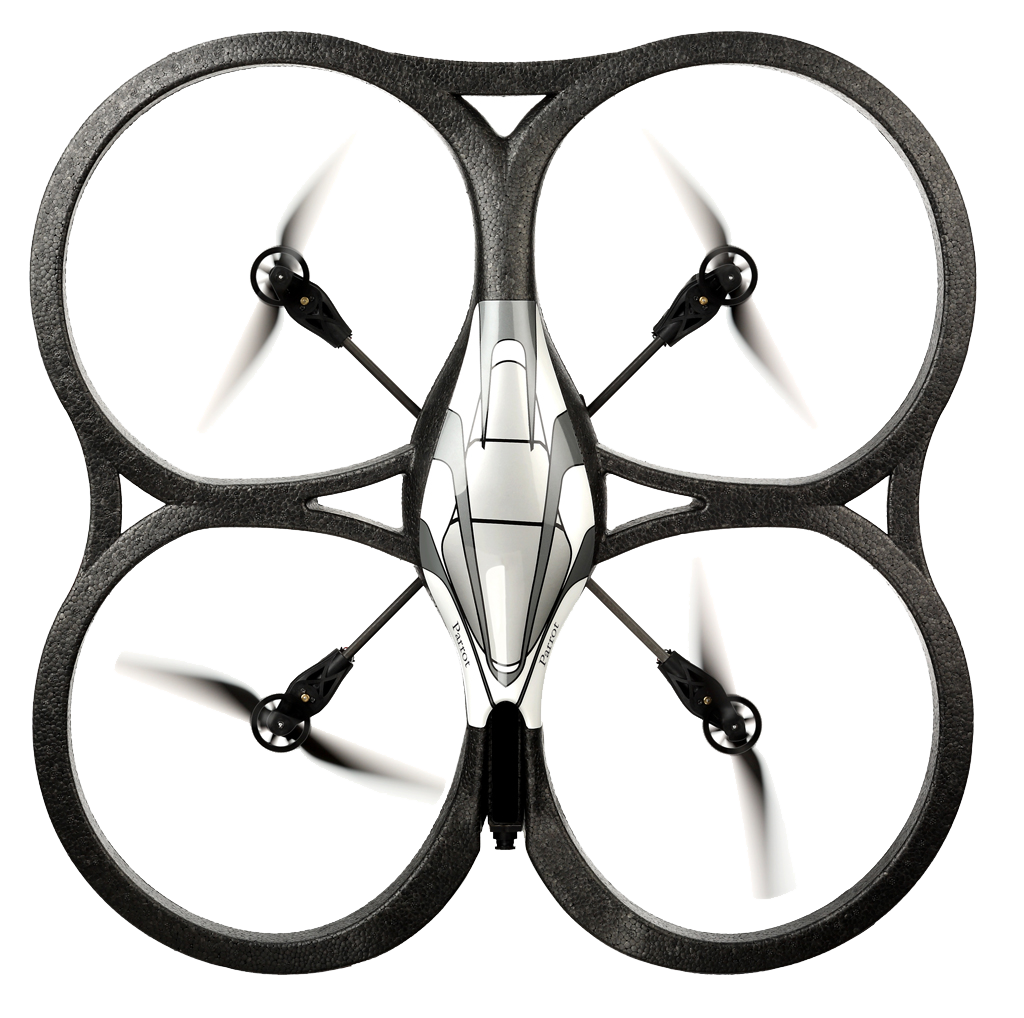
\includegraphics[scale=0.5, angle=-225]{figure/ARDrone_front.png}};
		
		\end{tikzpicture}
	\end{center}
	
\end{figure}

\section{Example \thedrawingOnImages}
\stepcounter{drawingOnImages}

	\begin{figure}[H]
	\begin{center}
		\scalebox{0.85}{			
			\begin{tikzpicture}
			\node (stazioneTerra) at (-4,0) {\includegraphics[scale=0.25]{figure/stazioneTerra.png}};
			\node (drone) at (2.5,0) {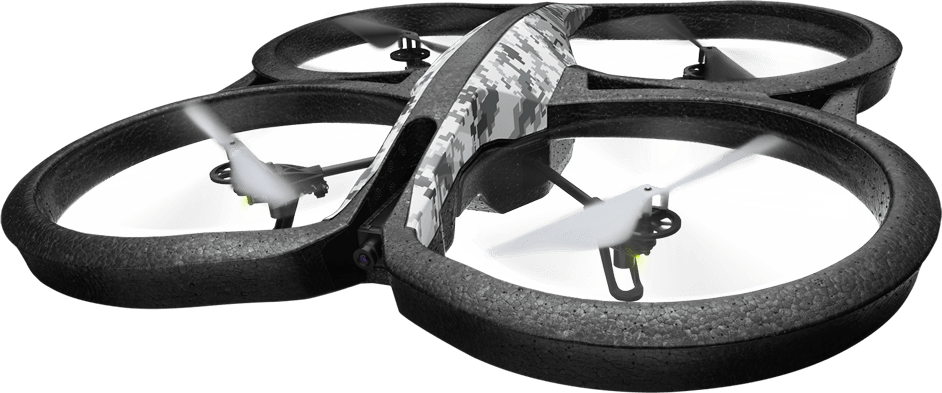
\includegraphics[scale=0.2]{figure/droneSnow.png}};
			\node (drone) at (-0.5,2.8) {\includegraphics[scale=0.2]{figure/Freccia_rossa.png}};
			\node (drone) at (-0.5,-2.8) {\includegraphics[scale=0.2]{figure/Freccia_blu.png}};	
			\end{tikzpicture}	
		}
	\end{center}
\end{figure}


\section{Example \thedrawingOnImages}
\stepcounter{drawingOnImages}

\begin{figure}[H]
	\begin{center}
		\begin{tikzpicture}
		\node (grafico) at (0,0) [text centered]{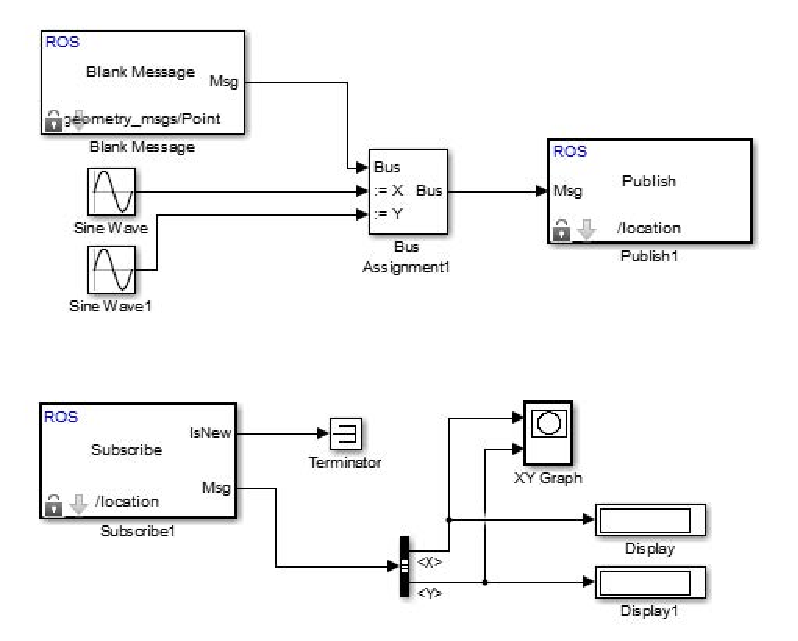
\includegraphics[scale=0.85]{pdf/intro_subsub_msgs}};
		
		\node (cornice1) at (0,2.15) [draw, rectangle, dashed, text centered, red!75, minimum height=4.75cm, minimum width=12cm, line width=2.5pt]{};
		
		\node (cornice2) at (0,-2.75) [draw, rectangle, dashed, text centered, green!75, minimum height=4cm, minimum width=12cm, line width=2.5pt]{};
		\end{tikzpicture}
	\end{center}

\end{figure}

\section{Example \thedrawingOnImages}
\stepcounter{drawingOnImages}

\begin{figure}[H]
	\begin{center}
			\begin{tikzpicture}
			
			%Rappresento gli angoli sul sistema assi-corpo
			\draw[latex-] (0.25,2.3) arc (-25:-110:0.30cm) node[above left]{$\psi$};
			\draw[latex-] (-1.0,-0.9) arc (45:-110:0.30cm);
			\draw (-1.0,-0.9) node[below right]{$\phi$};
			\draw[latex-] (1.825,-0.2) arc (105:-70:0.30cm);
			\draw (2.05,-0.25) node[right]{$\theta$};
			
			%Inserisco il sistema di riferimento assi-corpo
			\draw[-latex] (0.05,0) coordinate -- (0.05,3) coordinate node[anchor=west]{$e_{z}$};
			\draw[-latex] (0.05,0) coordinate -- (-1.60,-1.55) coordinate node[left]{$e_{x}$};
			\draw[-latex] (0.05,-0.1) coordinate -- (2.55,-0.6) coordinate node[below right]{$e_{y}$};
			\draw (0.05,0.8) node[below right]{$O_{ABC}$};
			
			%Inserisco il quadricottero
			\node (esacottero) at (0,0) [text centered]{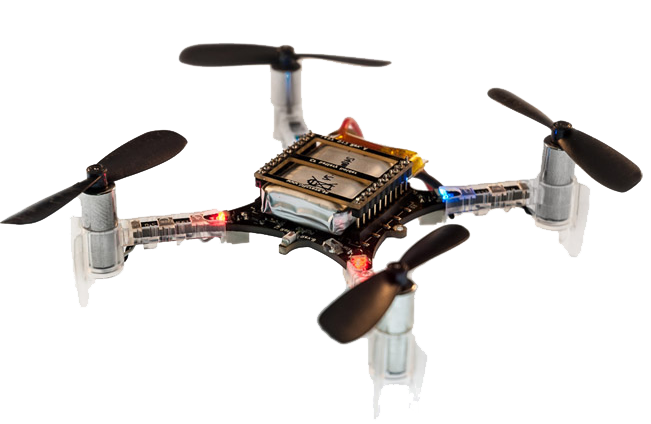
\includegraphics[scale=0.2]{figure/Crazyflie20_1.png}};
			
			%Inserisco gli archi per le Omega
			\draw[-latex] (-1.3,0.655) arc (55:-15:0.35cm); %omega 1
			\draw[latex-] (-0.05,1.225) arc (-25:-120:0.30cm); %omega 2
			\draw[-latex] (1.2,0.87) arc (55:-15:0.35cm); %omega 3
			\draw[latex-] (0.6225,0.125) arc (-25:-120:0.30cm); %omega 4
			
			%Disegno i vettori delle forze
			\draw[-latex] (-1.225,0.3) coordinate -- (-1.225,0.9) node[left]{$\omega_1$};
			\draw[-latex] (-0.21,0.9) coordinate -- (-0.21,1.5) node[left]{$\omega_2$};
			\draw[-latex] (1.26,0.525) coordinate -- (1.26,1.125) node[right]{$\omega_3$};
			\draw[-latex] (0.36,-0.25) coordinate -- (0.36,0.35) coordinate;
			\draw (0.85,-0.7225) node[above]{$\omega_4$};
			
			%Rappresento gli angoli sul sistema di riferimento inerziale
			\draw[latex-] (-2.9,-2.5) arc (-25:-110:0.30cm) node[left]{$\psi$};
			\draw[latex-] (-2.475,-5.9) arc (105:-70:0.30cm);
			\draw (-2.15,-6.15) node[right]{$\theta$};
			\draw[latex-] (-5.4,-4.9) arc (45:-130:0.30cm);
			\draw (-5.6,-5.3) node[below right]{$\phi$};
			
			%Inserisco il sistema di riferimento inerziale
			\draw[-latex] (-3.05,-5) coordinate -- (-3.05,-2) coordinate node[anchor=east]{$e_{z}$};
			\draw[-latex] (-3.05,-5) coordinate -- (-6.05,-5.275) coordinate node[above right]{$e_{x}$};
			\draw[-latex] (-3.05,-5) coordinate -- (-2.25,-6.725) coordinate node[below left]{$e_{y}$};
			\draw (-3.05,-5) node[right]{$O_{FI}$};
			
			\end{tikzpicture}
	\end{center}
\end{figure} 


\section{Example \thedrawingOnImages}
\stepcounter{drawingOnImages}


	\begin{figure}[H]
	\begin{center}
		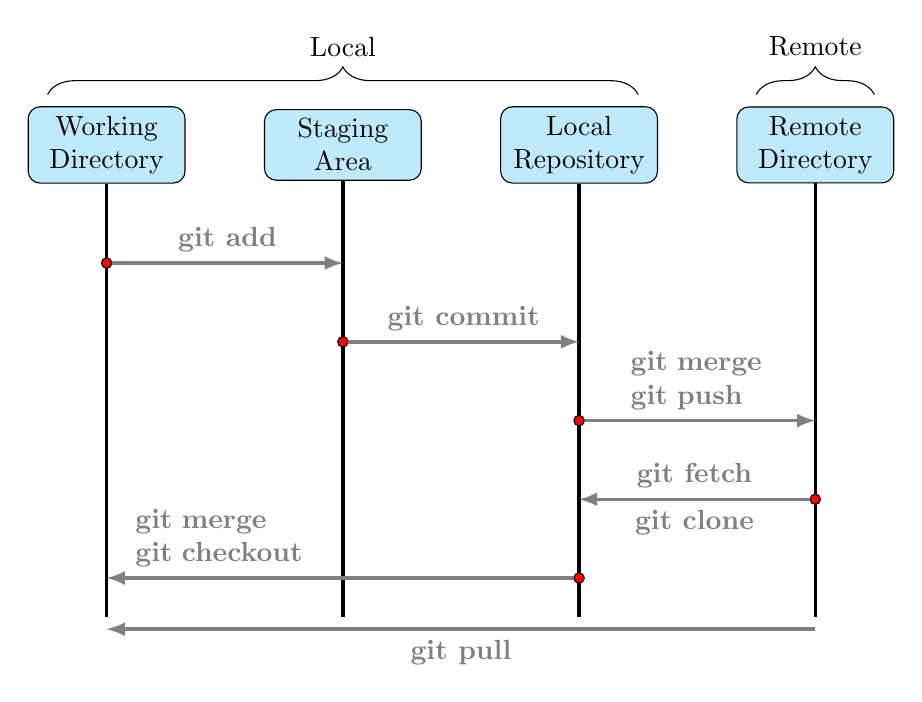
\begin{tikzpicture}
		
		%Rappresento i blocchi
		\node(WorkingDirectory) at (0,0) [rounded corners=0.15cm, draw, minimum width=1.5cm, minimum height=0.75cm, rectangle, text centered, fill=cyan!25, text width=5em]{Working\\Directory};
		\node(StagingArea) at (3,0) [rounded corners=0.15cm, draw, minimum width=1.5cm, minimum height=0.75cm, rectangle, text centered, fill=cyan!25, text width=5em]{Staging\\Area};
		\node(LocalRepository) at (6,0) [rounded corners=0.15cm, draw, minimum width=1.5cm, minimum height=0.75cm, rectangle, text centered, fill=cyan!25, text width=5em]{Local\\Repository};
		\node(RemoteDirectory) at (9,0) [rounded corners=0.15cm, draw, minimum width=1.5cm, minimum height=0.75cm, rectangle, text centered, fill=cyan!25, text width=5em]{Remote\\Directory};
		
		%Rappresento i collegamenti
		\draw[-, line width=1.25pt] (WorkingDirectory.south) -- (0,-6);
		\draw[-, line width=1.25pt] (StagingArea.south) -- (3,-6);
		\draw[-, line width=1.25pt] (LocalRepository.south) -- (6,-6);
		\draw[-, line width=1.25pt] (RemoteDirectory.south) -- (9,-6);
		
		%Inserisco le bubble
		\node (bubble1) at (0,-1.5) [circle, draw, scale=0.4, fill=red]{};
		\node (bubble2) at (3,-2.5) [circle, draw, scale=0.4, fill=red]{};
		\node (bubble3) at (6,-3.5) [circle, draw, scale=0.4, fill=red]{};
		\node (bubble4) at (9,-4.5) [circle, draw, scale=0.4, fill=red]{};
		\node (bubble5) at (6,-5.5) [circle, draw, scale=0.4, fill=red]{};
		
		%Rappresento i collegamenti
		\draw[-latex, gray, line width=1.25pt] (bubble1) -- node[above]{\textbf{git add}} (3,-1.5) coordinate;
		\draw[-latex, gray, line width=1.25pt] (bubble2) -- node[above]{\textbf{git commit}} (6,-2.5) coordinate;
		\draw[-latex, gray, line width=1.25pt] (bubble3) -- node[above, text width=5em]{\textbf{git merge\\git push}} (9,-3.5) coordinate;
		\draw[-latex, gray, line width=1.25pt] (bubble4) -- node[above]{\textbf{git fetch}} node[below]{\textbf{git clone}} (6,-4.5) coordinate;
		\draw[-latex, gray, line width=1.25pt] (bubble5) -- node[above left, text width=7em]{\textbf{git merge\\git checkout}} (0,-5.5) coordinate;
		\draw[-latex, gray, line width=1.25pt] (9,-6.15) coordinate -- node[below]{\textbf{git pull}} (0,-6.15) coordinate;
		
		%Disegno le parentesi graffe - blocco virtual world
		\draw [decorate,decoration={brace, amplitude=10pt,raise=4pt},yshift=0pt] (-0.75,0.5) -- (6.75,0.5) node [black,midway,xshift=0.0cm,yshift=0.75cm] {Local};
		\draw [decorate,decoration={brace, amplitude=10pt,raise=4pt},yshift=0pt] (8.25,0.5) -- (9.75,0.5) node [black,midway,xshift=0.0cm,yshift=0.75cm] {Remote};
		
		\end{tikzpicture}
	\end{center}
\end{figure}
